\chapter{BACKGROUND}
\minitoc
% \newpage
\section{General introduction}
Lorem ipsum dolor sit amet, consectetur adipiscing elit, sed do eiusmod tempor incididunt ut labore et dolore magna aliqua. Amet nulla facilisi morbi tempus iaculis urna id volutpat lacus. Nisl nisi scelerisque eu ultrices vitae auctor. Nisi scelerisque eu ultrices vitae auctor eu augue. Orci sagittis eu volutpat odio. Dolor purus non enim praesent elementum facilisis leo. Ultrices neque ornare aenean euismod. Consectetur libero id faucibus nisl tincidunt. At auctor urna nunc id cursus. Turpis cursus in hac habitasse platea dictumst quisque. Id aliquet risus feugiat in ante metus dictum. Risus viverra adipiscing at in tellus integer feugiat scelerisque. Arcu non odio euismod lacinia at quis risus. Eget magna fermentum iaculis eu non diam phasellus. Cras semper auctor neque vitae tempus quam pellentesque nec. Ultrices gravida dictum fusce ut placerat orci nulla pellentesque dignissim. Massa sapien faucibus et molestie ac feugiat. Magna fringilla urna porttitor rhoncus dolor purus non enim. Amet massa vitae tortor condimentum lacinia quis vel eros. At varius vel pharetra vel turpis nunc eget.

\subsection{The electromagnetic spectrum}
\textbf{Light} is usually interpreted as the \textit{visible light}; that's because it is what can be perceived by the eye, but that changed in the 1800s when it was discovered that light was a more general phenomenon; and it is more common to use \textbf{electromagnetic radiation} when referring to light in its various forms \citep{ball2007}.

The electromagnetic spectrum is the \textbf{range} of electromagnetic radiations.

The \hyperref[fig:em-spec]{figure \ref{fig:em-spec}} shows important properties and relations between different radiations of the electromagnetic spectrum. The order of these radiations in increasing wavelength is: Gamma-rays $\gamma$, X-rays, Ultra-Violer, Visible, Infrared, Micro-waves, Radio-waves.

The infrared portion of the electromagnetic spectrum is usually divided into three sub-regions; the \textit{near}-, \textit{mid}- and \textit{far}-infrared, named for their relation to the visible spectrum.

\begin{figure}[ht]
	\centering
	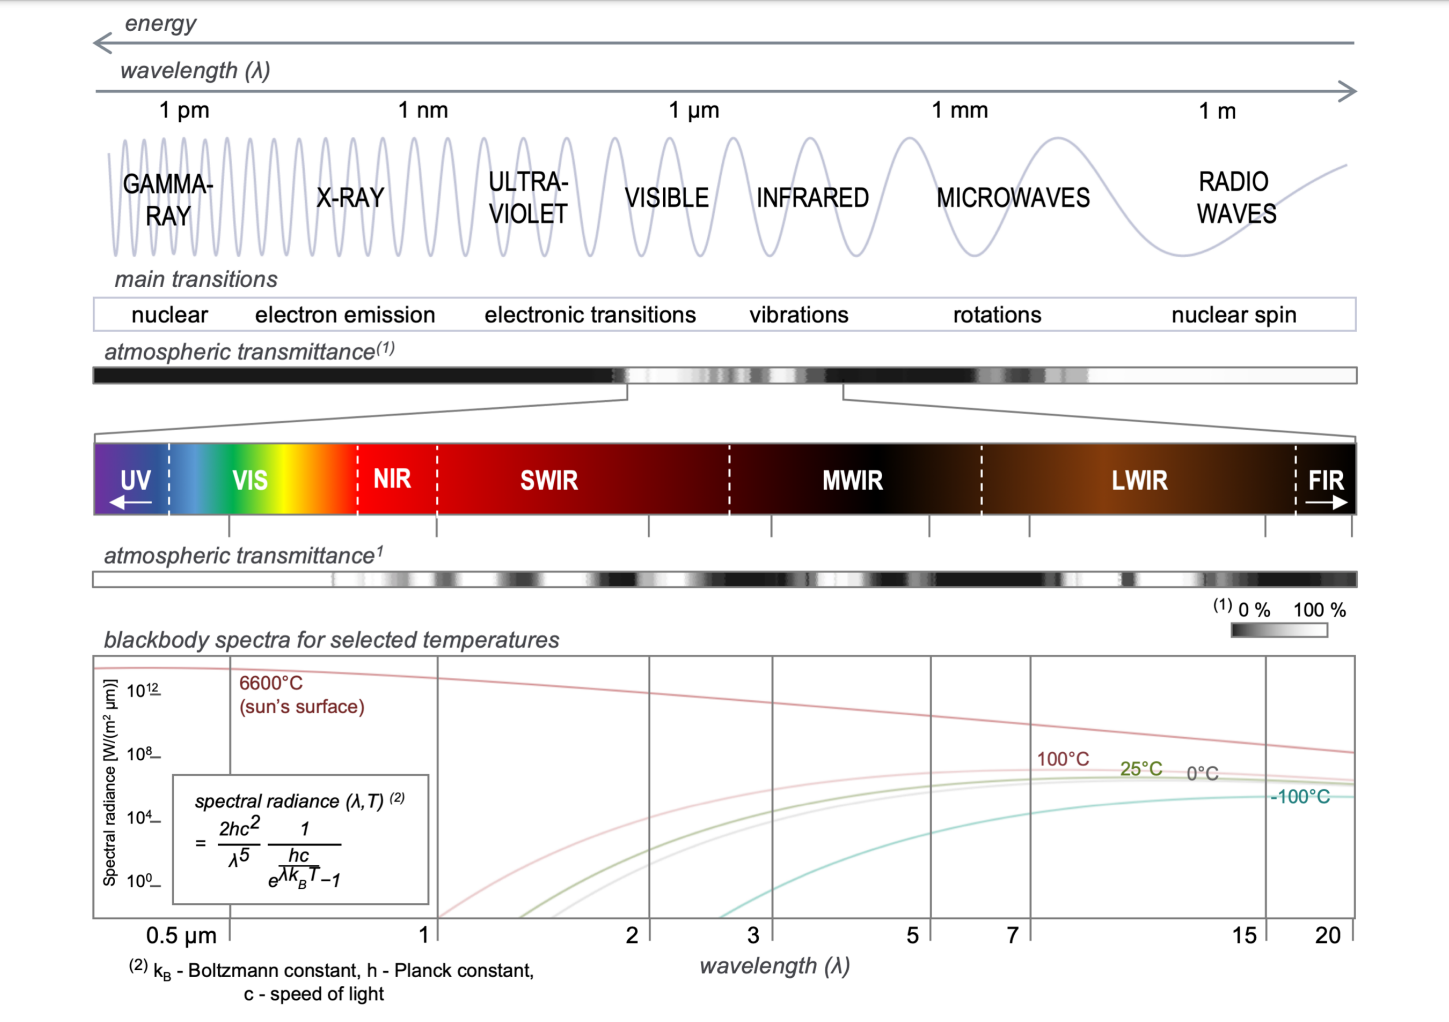
\includegraphics[width=.95\textwidth]{electromagn-spectrum.png}  
	\caption{The electromagnetic spectrum \citep{lorenz2019}}
	\label{fig:em-spec}
\end{figure}

\subsection{Lorem Ipsum 1}
\subsection{Lorem Ipsum 1}
\subsection{Lorem Ipsum 1}
\section{Lorem Ipsum 1}
\subsection{Lorem Ipsum 1}
\subsection{Lorem Ipsum 1}
\section{Lorem Ipsum 1}
\subsection{Lorem Ipsum 1}
\subsubsection{Lorem Ipsum 1}
\section{Lorem Ipsum 1}
\subsection{Lorem Ipsum 1}
\subsection{Lorem Ipsum 1}
\subsubsection{Lorem Ipsum 1}
\section{Lorem Ipsum 1}
\section{Lorem Ipsum 1}
